\documentclass[10pt]{article}

% ---- NeurIPS style ----
\usepackage{neurips_2026}

% ---- Packages ----
\usepackage[utf8]{inputenc}
\usepackage[T1]{fontenc}
\usepackage{amsmath,amssymb,amsfonts}
\usepackage{graphicx}
\usepackage{booktabs}
\usepackage{hyperref}
\usepackage{natbib}
\usepackage{xcolor}
\usepackage{multirow}
\usepackage{subcaption}
\usepackage{algorithm}
\usepackage{algorithmic}
\usepackage{microtype}

% Allow more floats per page
\renewcommand{\topfraction}{0.85}
\renewcommand{\textfraction}{0.1}
\setcounter{topnumber}{3}

\hypersetup{
  colorlinks=true,
  linkcolor=blue!70!black,
  citecolor=green!50!black,
  urlcolor=blue!70!black
}

% ---- Custom commands ----
\newcommand{\method}{positional distillation}
\newcommand{\Method}{Positional distillation}
\newcommand{\methodfull}{Positional Distillation}
\newcommand{\posN}{\text{pos-}N}
\newcommand{\KL}{\mathrm{KL}}
\newcommand{\bboxed}{\texttt{\textbackslash boxed\{\}}}
\newcommand{\tbd}[1]{\textcolor{red}{[TBD: #1]}}

\title{\textbf{On the Token Reward Quality of On-Policy Distillation}}

\author{
  Anonymous Authors
}

\date{}

\begin{document}

\maketitle

% ============================================================================
% ABSTRACT
% ============================================================================
\begin{abstract}
On-policy knowledge distillation trains the student on its own rollouts while the teacher provides token-level soft targets. A common assumption is that the teacher's supervision is uniformly useful across all token positions. We show this assumption is wrong: teacher signal quality varies dramatically by position. At early positions, the teacher provides an independent assessment of reasoning strategy (entropy 1.07, 42\% token-level disagreement with the student); at later positions, the teacher is conditioned on the student's prefix and largely rubber-stamps the student's choices (entropy 0.14, 13\% disagreement). Training on only the first 100 tokens improves performance by +14.9pp over baseline, while training on the middle or last 100 tokens \emph{decreases} performance below baseline. This reveals that later-position supervision is not merely uninformative---it is actively harmful. We propose \emph{positional distillation}: restricting KD loss to the first $N$ response tokens, yielding a 20--35$\times$ wall-clock speedup. Experiments across math reasoning (MATH-500), code generation (HumanEval/MBPP), and function calling (BFCL), with multiple teacher scales (1.7B--8B) and model families (Qwen, Gemma), show that positional distillation matches or exceeds full-sequence distillation while eliminating training instability.
\end{abstract}

% ============================================================================
% 1. INTRODUCTION
% ============================================================================
\section{Introduction}
\label{sec:intro}

On-policy knowledge distillation (KD) trains the student on its own rollouts while the teacher supplies token-level soft targets~\citep{agarwal2024onpolicy, gu2024minillm}. From the student's perspective, this is equivalent to receiving a \emph{dense, token-level reward}: at every position the teacher acts as a reward model, scoring each student-generated token via its conditional distribution~\citep{gu2024minillm, lu2025onpolicy, yang2026beyond}. A natural assumption is that this token reward is uniformly useful across positions---that every token in the student's trajectory receives an equally valuable signal from the teacher. This paper challenges that assumption.

This token reward is typically understood as the teacher assessing the quality of the student's answer given the question. But since the reward is computed autoregressively---$p_\text{teacher}(y_t \mid x, y_{<t})$, where $y_{<t}$ is the \emph{student's own prefix}---the interaction between teacher and student naturally decomposes into two regimes. At \textbf{early positions}, the prefix is largely determined by the prompt $x$, so the teacher's assessment is primarily based on the question itself---an \emph{independent} evaluation. At \textbf{later positions}, the teacher is conditioned on hundreds of student-generated tokens; it is no longer evaluating the student based on the question alone, but rather scoring how to continue \emph{this particular} student trajectory---a \emph{dependent} evaluation shaped by the student's prior choices. These two regimes are fundamentally different in nature. This raises a critical question: \emph{is the teacher's token reward at later positions still high quality?} We investigate this question and find that the answer is no.

Our analysis reveals several converging lines of evidence. \textbf{(1) Signal strength decays with position.} Teacher entropy drops from 1.07 at early positions to 0.14 at late positions; teacher-student agreement rises from 58\% to 87\%. At later positions, the teacher is effectively rubber-stamping the student's choices. \textbf{(2) Later-position supervision is actively harmful.} Training on the first 100 tokens improves MATH-500 accuracy by +14.9pp over baseline, while training on the middle or last 100 tokens \emph{decreases} accuracy by 1--4pp below baseline. \textbf{(3) Full-sequence training degrades over time.} On coding tasks, full-sequence distillation degrades from 40.2\% to 26.8\% HumanEval---consistent with accumulated exposure to low-quality late-position signals.

These findings motivate \textbf{\methodfull{}}: restricting KD loss to the first $N$ response tokens and truncating rollouts accordingly. This is not merely an efficiency trick---it is a principled response to the non-uniform signal quality we identify. Experiments across math reasoning (MATH-500), code generation (HumanEval/MBPP), and function calling (BFCL), with teacher scales from 1.7B to 8B and cross-family validation (Qwen, Gemma), show that positional distillation matches or exceeds full-sequence distillation on all tasks while providing 20--35$\times$ wall-clock speedup and eliminating training instability.

Our contributions are:
\begin{enumerate}
    \item \textbf{Analysis of teacher signal quality.} We show that in on-policy KD, the teacher's supervision quality degrades along the trajectory: early tokens carry strong, independent signal about reasoning strategy, while later tokens contribute weak, dependent signal that is actively harmful when trained on (Section~\ref{sec:analysis}).
    \item \textbf{\methodfull{}.} A method that restricts KD loss to the first $N$ response tokens, simultaneously improving quality, stability, and efficiency (Section~\ref{sec:method}).
    \item \textbf{Broad evaluation.} Consistent improvements across three tasks, three teacher scales, and two model families, with detailed ablations on position selection and training dynamics (Section~\ref{sec:experiments}).
\end{enumerate}


% ============================================================================
% 2. SIGNAL QUALITY ANALYSIS
% ============================================================================
\section{Token Reward Quality Analysis by Position}
\label{sec:analysis}

We analyze the quality of the teacher's per-token supervision signal across positions in student-generated trajectories. All analysis in this section uses Qwen2.5-Math-1.5B as the student and Qwen3-1.7B as the teacher on MATH-500, with 59,936 on-policy trajectories (mean length 386 tokens).

% ---- Figure Group 1: Signal Distribution (placed early for page 2 float) ----
\begin{figure*}[t]
    \centering
    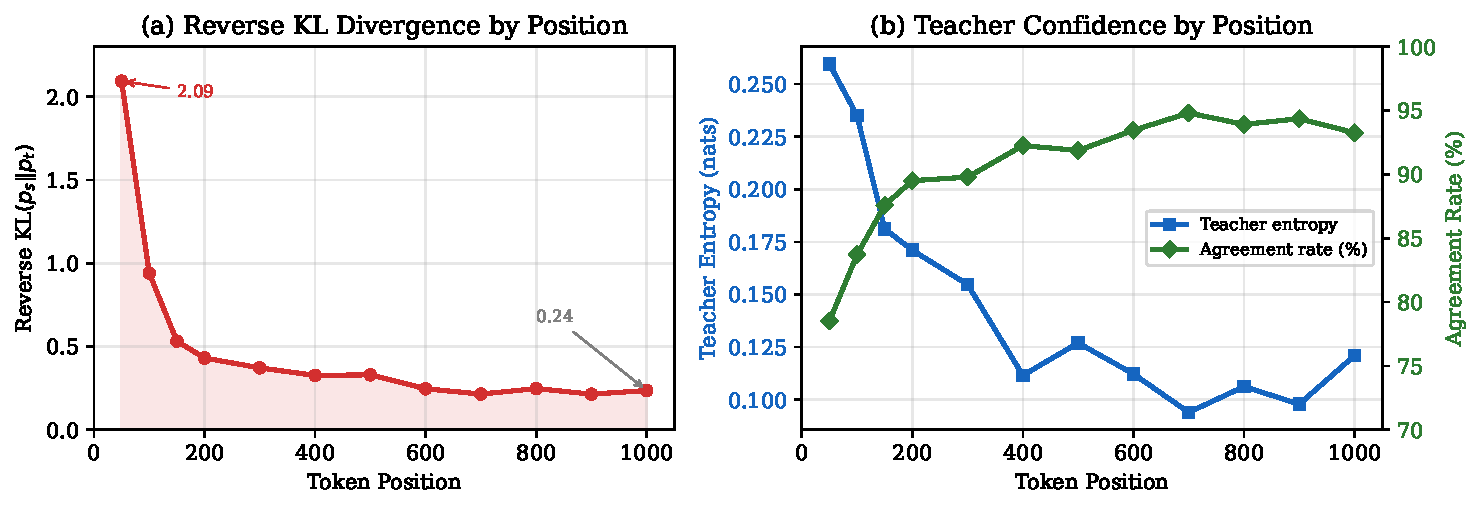
\includegraphics[width=\textwidth]{figures/fig_signal_reverse_kl.pdf}
    \caption{\textbf{Teacher signal quality degrades with position} (100 MATH-500 problems, 1 trajectory each). (a) Reverse KL divergence KL$(p_s \| p_t)$ decays from 2.09 in the first 50 tokens to $\sim$0.24 by position 1000. Dashed line shows the token-level log-prob gap, which nearly coincides with the reverse KL. (b) Teacher entropy drops from 0.26 to 0.12 while teacher-student agreement rises from 79\% to 93\%. At later positions, the teacher is effectively rubber-stamping the student's choices.}
    \label{fig:signal}
\end{figure*}

\subsection{The Conditional Scoring Problem}
\label{sec:conditional}

In on-policy distillation, the teacher scores position $t$ via $p_\text{teacher}(\cdot \mid x, y_{1:t-1}^\text{student})$. This score is \emph{not} the teacher's unconditional opinion about what token should come next---it is the teacher's opinion \emph{conditioned on the student's prefix}. As $t$ increases, the prefix $y_{1:t-1}$ becomes increasingly student-determined, and the teacher's scoring increasingly reflects ``how to continue this student trajectory'' rather than ``what is the right approach.''

This creates a \emph{phase shift} in the teacher's role along the trajectory. At early positions, the teacher acts as a \textbf{strategic guide}---providing independent judgment on how to approach the problem. At later positions, the teacher degenerates into a \textbf{syntax checker}---merely confirming that the student's execution is locally coherent within the student's chosen approach. If the student's strategy is suboptimal, the later-position signal teaches the student to better execute a suboptimal approach---rather than to choose a better one.


\subsection{Per-Position KL Distribution}
\label{sec:kl_distribution}

To investigate the distillation signal, we generate 59,936 on-policy trajectories (mean length 386 tokens) from the undistilled student and compute per-position KL divergence against the teacher. Positions are 0-indexed throughout (position 0 is the first generated token).

Figure~\ref{fig:signal} shows two complementary views of the signal distribution. The reverse KL divergence (left) reveals that the distillation signal is massively front-loaded: the first 50 tokens (KL = 2.09) carry 8.9$\times$ more signal than the 900--1000 range (KL = 0.24), with a steep initial decay followed by a long, slowly declining tail beyond position 200. The teacher confidence analysis (right) explains why: at early positions, the teacher's distribution has higher entropy (0.26 nats) and lower agreement with the student (79\%). By position 1000, entropy drops to 0.12 and agreement rises to 93\%---the teacher is no longer providing independent guidance, but merely confirming the student's choices.

This is a direct consequence of the conditional scoring problem (\S\ref{sec:conditional}): once the student's prefix determines the reasoning approach, the teacher's conditional distribution collapses to near-agreement. The residual disagreement at late positions is dominated by formatting conventions (LaTeX delimiters, code patterns) rather than reasoning content.

\paragraph{Strategy vs.\ execution.} Token-type analysis (Appendix~\ref{app:token_classification}) reveals that early high-KL tokens are predominantly \emph{planning} tokens (``To'', ``First'', ``Let'')---reflecting strategy disagreement---while late high-KL tokens are formatting conventions. Figure~\ref{fig:example} illustrates this with a concrete example: the first 100 tokens establish the solution approach, while the last 100 tokens execute the computation.

% ---- Figure 2: Example + Continuation/Bar chart (combined) ----
\begin{figure*}[!t]
\centering
\footnotesize
\fbox{\parbox{0.93\textwidth}{
\textbf{Problem:} In an isosceles right triangle, the altitude to the hypotenuse has length $4\sqrt{2}$. What is the area? \\[3pt]
\colorbox{blue!10}{\parbox{0.91\textwidth}{\textbf{First 100 tokens (strategy):} ``Let's start by understanding the problem. In an isosceles right triangle, the two legs are equal, and the hypotenuse is $\sqrt{2}$ times the leg. If we denote each leg by $a$, then hypotenuse $= a\sqrt{2}$. The altitude to the hypotenuse is half the leg, because the altitude bisects the...''}} \\[3pt]
\colorbox{orange!10}{\parbox{0.91\textwidth}{\textbf{Last 100 tokens (execution):} ``...altitude from the right-angle vertex to the hypotenuse. This altitude has length $h = \frac{a \cdot a}{a\sqrt{2}} = \frac{a^2}{a\sqrt{2}} = \frac{a}{\sqrt{2}} = \frac{a\sqrt{2}}{2}$. Setting this equal to $4\sqrt{2}$: $\frac{a\sqrt{2}}{2} = 4\sqrt{2}$, so $a\sqrt{2} = 8\sqrt{2}$, giving $a = 8$. The area is $\frac{1}{2} \times 8 \times 8 = \boxed{32}$.''}}
}}
\vspace{4pt}
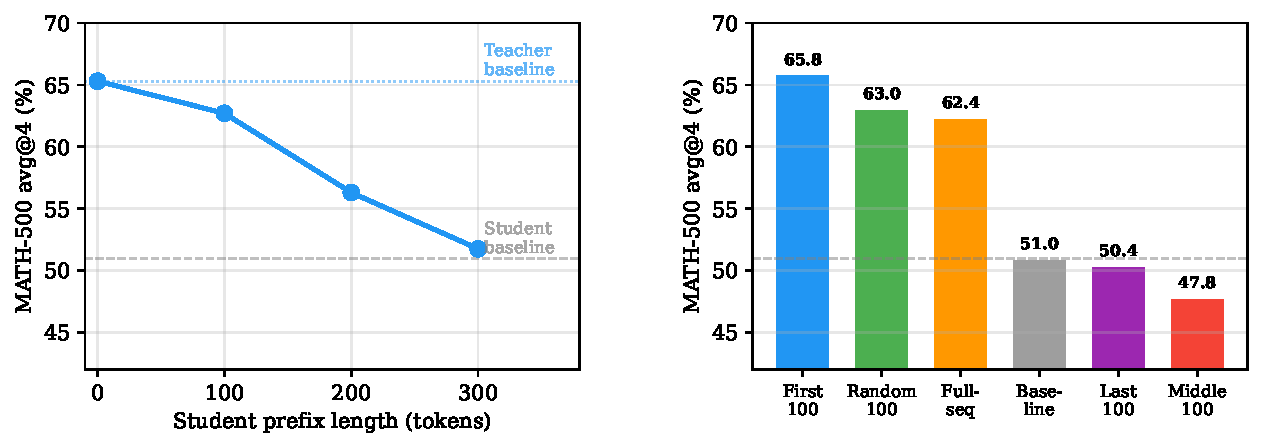
\includegraphics[width=0.95\textwidth]{figures/fig_analysis_4_degradation.pdf}
\vspace{-6pt}
\caption{\textbf{Early tokens encode strategy; later tokens merely execute.} \emph{Top:} example showing first 100 tokens (blue) establish the approach while last 100 tokens (orange) execute computation. \emph{Bottom left:} prefix continuation---teacher performance degrades to student baseline by 300 tokens. \emph{Bottom right:} best-checkpoint accuracy per 100-token region. First-100 yields +14.9pp; middle-100 and last-100 hurt.}
\label{fig:example}
\label{fig:continuation}
\end{figure*}

\subsection{Test-Time Validation: Prefix Continuation}
\label{sec:continuation}

We directly test whether early tokens determine response quality via prefix continuation (Figure~\ref{fig:continuation}, left). With a 100-token student prefix, the teacher achieves 62.70\% avg@4---only 2.6pp below its baseline. At 300 tokens, performance falls to 51.75\%, nearly matching the student baseline: the student's choices become entrenched. The rapid degradation quantifies the \emph{window of effective influence}: the first $\sim$100 tokens are where reasoning strategy is still malleable.

\subsection{Training-Time Validation: Position Region Ablation}
\label{sec:position_ablation}

The analysis above predicts that early-position training should be most effective and later-position training should be harmful. We test this by training on different 100-token regions (Figure~\ref{fig:continuation}, right).

First-100 improves avg@4 by +14.9pp and outperforms full-sequence training. Middle-100 and last-100 both perform \emph{below the undistilled baseline}---later-position signals are not merely uninformative, they are actively harmful. Random-100 (63.05\%) outperforms full-seq (62.35\%), further confirming that including later-position tokens is a net negative.


\subsection{Training Instability as a Consequence}
\label{sec:degradation}

Figure~\ref{fig:degradation} shows that full-sequence distillation degrades with continued training on coding (HumanEval drops from 40.2\% to 26.8\%, $-$33\%), while positional distillation remains stable. This is a direct consequence of the signal quality analysis: over many training steps, noisy gradients from later positions accumulate and distort the student's parameters.

\subsection{Summary of Findings}
\label{sec:hypothesis}

Our analysis reveals a coherent picture: (1) the teacher's signal is strong and independent at early positions, where reasoning strategy is being determined; (2) the signal decays to near-agreement at later positions, where the teacher is conditioned on the student's prefix; (3) training on later positions is harmful, and full-sequence degradation is a consequence of this harm. This motivates restricting distillation to early positions.


% ============================================================================
% 4. METHOD
% ============================================================================
\section{Method: Positional Distillation}
\label{sec:method}

\subsection{Formulation}

In standard on-policy reverse KL distillation, the student $p_\theta$ generates a response $\mathbf{x} = (x_1, \ldots, x_T)$ conditioned on a prompt, and the loss is computed against the teacher $q_\phi$:
\begin{equation}
\mathcal{L}_{\text{full}} = \mathbb{E}_{\mathbf{x} \sim p_\theta} \left[ \sum_{t=1}^{T} \KL\!\left(q_\phi(\cdot \mid \mathbf{x}_{<t}) \;\|\; p_\theta(\cdot \mid \mathbf{x}_{<t})\right) \right].
\label{eq:full_loss}
\end{equation}

\Method{} restricts the loss to the first $N$ response tokens:
\begin{equation}
\mathcal{L}_{\text{pos}} = \mathbb{E}_{\mathbf{x} \sim p_\theta} \left[ \sum_{t=1}^{N} \KL\!\left(q_\phi(\cdot \mid \mathbf{x}_{<t}) \;\|\; p_\theta(\cdot \mid \mathbf{x}_{<t})\right) \right],
\label{eq:pos_loss}
\end{equation}
where $N$ is a fixed position cutoff ($N \ll T$ in practice). If the student generates an EOS token before position $N$, loss is computed only up to EOS.

In practice, we both restrict the loss \emph{and} truncate the rollout to $N$ tokens. This couples two benefits: loss masking avoids low-quality tail positions (stability), while rollout truncation reduces generation cost (efficiency). Since autoregressive generation is the dominant cost in on-policy KD, truncating from $T{\sim}400$ to $N{=}100$ tokens yields 20--35$\times$ wall-clock speedup (Table~\ref{tab:timing}).


% ============================================================================
% 4. GENERALIZATION EXPERIMENTS
% ============================================================================
\section{Generalization Experiments}
\label{sec:experiments}

\subsection{Setup}

\paragraph{Models.} We evaluate across multiple student-teacher pairs. Our primary student is Qwen2.5-Math-1.5B~\citep{qwen2024qwen25math}, paired with teachers of increasing scale: Qwen3-1.7B, Qwen3-4B, and Qwen3-8B~\citep{qwen2025qwen3}. To test cross-family generality, we also evaluate with gemma-2-2b-it (student) and gemma-3-4b-it (teacher), which use different tokenizers requiring cross-tokenizer re-tokenization and shared-vocabulary KL computation.

\paragraph{Training.} All experiments use LoRA~\citep{hu2022lora} ($r{=}32$, $\alpha{=}64$, all linear layers, lr = $5{\times}10^{-5}$) with reverse KL divergence loss. Temperature 0.7 for on-policy generation. Each training step processes a batch of 16 problems with 1 rollout per problem ($n_{\text{samples}}{=}1$, batch size 16). We train for 200 steps on math and function calling, 400 steps on coding, saving checkpoints every 50 steps. Training data: 3,200 math problems, 6,400 coding problems (CodeUltraFeedback), and 3,200 function calling examples (glaive-function-calling-v2). Our method uses $N{=}100$ unless otherwise specified.

\paragraph{Evaluation.} MATH-500~\citep{hendrycks2021measuring, lightman2023verify} with $n{=}4$ samples at temperature 0.7 (reporting avg@4). HumanEval/HumanEval+ and MBPP/MBPP+~\citep{chen2021evaluating, austin2021program, liu2024evalplus} at temperature 0.0 (reporting pass@1). BFCL~\citep{yan2024bfcl} with 600 problems (reporting full accuracy: correct function name and arguments).

\subsection{Main Results}

Table~\ref{tab:main_results} presents the unified main results across tasks, teacher scales, and model families. We report the best performance achieved across all training steps for each configuration.

\begin{table}[t]
\centering
\caption{\textbf{Main results.} Best performance across training steps for each configuration. \textbf{Bold}: best per teacher. Full-seq results use the best step before degradation. Time: seconds per training step (gen + score + train). Gemma uses gemma-2-2b-it student $\rightarrow$ gemma-3-4b-it teacher.}
\label{tab:main_results}
\footnotesize
\begin{tabular}{ll cccc c}
\toprule
\textbf{Teacher} & \textbf{Method} & \textbf{MATH-500} & \textbf{HumanEval} & \textbf{MBPP} & \textbf{BFCL} & \textbf{Time} \\
 & & avg@4 & pass@1 & pass@1 & full\_acc & (s/step) \\
\midrule
\multicolumn{7}{l}{\textit{Student: Qwen2.5-Math-1.5B (LoRA)}} \\
\midrule
--- & Baseline & 50.95 & 32.93 & 52.12 & 2.70 & --- \\
\midrule
\multirow{3}{*}{Qwen3-1.7B} & Full-seq & 62.35 & 40.24 & 52.65 & --- & ${\sim}$280 \\
 & \textbf{Ours ($N{=}50$)} & \textbf{66.65} & \textbf{42.07} & 52.12 & 57.20 & ${\sim}$4 \\
 & \textbf{Ours ($N{=}100$)} & 65.85 & \textbf{42.07} & 49.21 & \textbf{61.30} & ${\sim}$8 \\
\midrule
\multirow{3}{*}{Qwen3-4B} & Full-seq & 67.45 & 39.63 & 50.79 & 34.83 & ${\sim}$210 \\
 & \textbf{Ours ($N{=}50$)} & --- & --- & --- & \textbf{50.17} & ${\sim}$4 \\
 & \textbf{Ours ($N{=}100$)} & \textbf{68.95} & \textbf{43.29} & \textbf{52.38} & 45.80 & ${\sim}$8 \\
\midrule
\multicolumn{7}{l}{\textit{Student: gemma-2-2b-it (LoRA) --- cross-family}} \\
\midrule
--- & Baseline & 13.45 & 23.78 & 40.48 & 73.50 & --- \\
\midrule
\multirow{3}{*}{gemma-3-4b-it} & Full-seq & 11.70$^\S$ & --- & --- & --- & ${\sim}$210 \\
 & \textbf{Ours ($N{=}50$)} & --- & --- & --- & --- & ${\sim}$4 \\
 & \textbf{Ours ($N{=}100$)} & \textbf{27.20} & \textbf{31.10} & \textbf{50.53} & \textbf{82.50} & ${\sim}$8 \\
\bottomrule
\multicolumn{7}{l}{\footnotesize $^\S$ Gemma full-seq degrades below baseline; other tasks not evaluated.}
\end{tabular}
\end{table}

\paragraph{Results.} With the Qwen3-1.7B teacher, \method{} matches or exceeds full-sequence distillation on all benchmarks while achieving 35--70$\times$ speedup. $N{=}50$ achieves the best math accuracy (66.65\% avg@4, +4.3pp over full-seq) and matches full-seq on MBPP; $N{=}100$ achieves the best BFCL score (61.30\%). Scaling to the 4B teacher improves quality further: 68.95\% avg@4 on math (+3.1pp over 1.7B), with \method{} outperforming full-seq on all metrics. The Gemma cross-family pair demonstrates that \method{} transfers across model families with incompatible tokenizers, doubling math accuracy (13.45\% $\rightarrow$ 27.20\%) and substantially improving all other metrics. Additional teacher scales (8B) are in Appendix~\ref{app:additional_pairs}.

\paragraph{Cascade effect.} A natural concern is that distilling only the first $N$ tokens might only improve those positions. We find the opposite: early-token distillation creates a \emph{cascade effect} that reshapes the entire response (Figure~\ref{fig:cascade}). Because the early tokens determine the reasoning strategy, improving them causes the subsequent execution tokens to change accordingly---even though those later positions receive zero distillation signal. Concretely, pos-200 reduces KL by 50--58\% within the trained range (positions 0--200) and by 35--39\% in the \emph{untrained} range (positions 200--400). This is consistent with the strategy-then-execution structure identified in Section~\ref{sec:kl_distribution}: better strategy decisions at early positions naturally lead to better execution at later positions.

\begin{figure}[t]
    \centering
    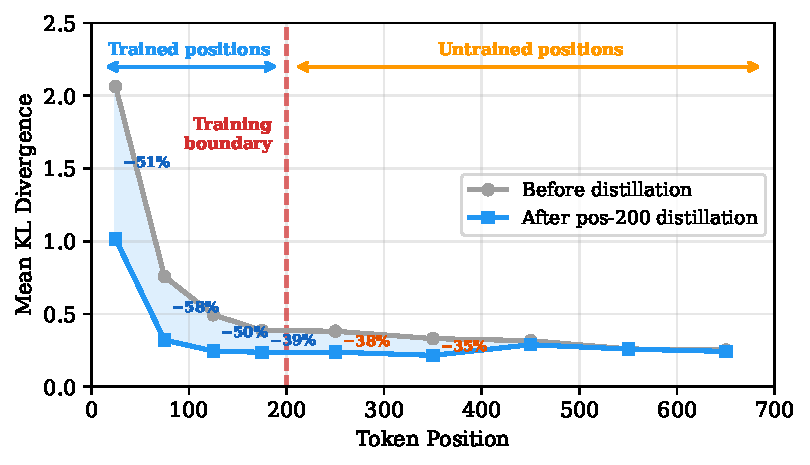
\includegraphics[width=\columnwidth]{figures/fig_cascade.pdf}
    \caption{\textbf{Cascade effect.} Pos-200 distillation reduces KL not only in the trained range (0--200) but also in the untrained range (200--400+), confirming that early-token improvements cascade through the autoregressive generation.}
    \label{fig:cascade}
\end{figure}


\subsection{Training Stability}
\label{sec:stability}

As shown in Figure~\ref{fig:degradation} and discussed in Section~\ref{sec:degradation}, full-sequence distillation degrades over training while \method{} remains stable. This is one of the three key advantages of positional distillation: better performance, no degradation, and dramatically faster training.


\subsection{Efficiency}
\label{sec:efficiency}

\begin{table}[t]
\centering
\caption{\textbf{Training resource usage for \method{} ($N{=}100$).} Peak GPU memory (measured via \texttt{nvidia-smi}) and per-step time breakdown. Student: Qwen2.5-Math-1.5B (LoRA), Teacher: Qwen3-1.7B. Each model on a separate GPU.}
\label{tab:timing}
\small
\begin{tabular}{l cc l}
\toprule
\textbf{Model} & \multicolumn{2}{c}{\textbf{Peak GPU Memory}} & \textbf{Time / step} \\
\cmidrule(lr){2-3}
 & bs$=$1 & bs$=$8 & \\
\midrule
Student (1.5B) & 4.9\,GB & 13.4\,GB & Gen:\;${\sim}$5\,s \quad Train:\;${\sim}$2\,s \\
Teacher (1.7B) & 4.6\,GB & 4.9\,GB & Scoring:\;${\sim}$1\,s \\
\bottomrule
\end{tabular}
\end{table}

\begin{figure}[t]
    \centering
    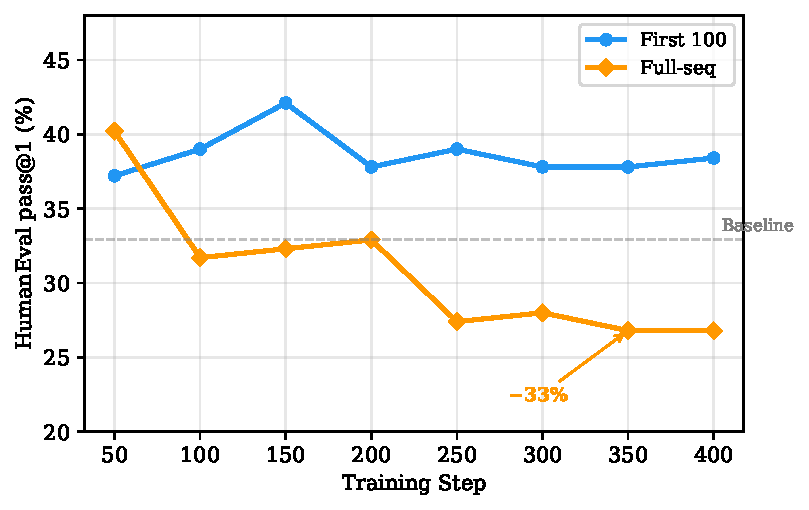
\includegraphics[width=0.7\columnwidth]{figures/fig_analysis_3_positions.pdf}
    \caption{\textbf{Full-sequence distillation degrades on coding.} On HumanEval, full-seq drops from 40.2\% to 26.8\% ($-$33\%) over 400 training steps, while first-100 positional distillation remains stable above baseline.}
    \label{fig:degradation}
\end{figure}

Table~\ref{tab:timing} shows the resource footprint of \method{}. The total per-step time is ${\sim}$8\,s (5\,s generation + 2\,s training + 1\,s teacher scoring), compared to ${\sim}$280\,s for full-seq distillation---a 35$\times$ speedup. Peak GPU memory with bs$=$8 is 13.4\,GB for the student and 4.9\,GB for the teacher, well within a single consumer GPU. \Method{} does not require a vLLM/SGLang inference server since 100 tokens can be generated via standard HF \texttt{generate}.

% ============================================================================
% 5. ABLATION EXPERIMENTS
% ============================================================================
\section{Ablation Experiments}
\label{sec:ablation}

\subsection{Position Limit Sweep}
\label{sec:pos_sweep}

How sensitive is \method{} to the choice of $N$? Figure~\ref{fig:pos_sweep} shows best avg@4 across $N \in \{5, 10, 20, 50, 100, 150, 200\}$ on MATH-500.

\begin{figure}[t]
    \centering
    
\includegraphics[width=0.75\columnwidth]{figures/fig_pos_sweep.pdf}
    \caption{\textbf{Position limit sweep on MATH-500.} Best avg@4 across training steps for each $N$. Performance increases monotonically and surpasses full-seq (dashed orange) at $N{\geq}150$. Even $N{=}5$ provides +5.5pp over baseline (dashed gray).}
    \label{fig:pos_sweep}
\end{figure}

The results reveal a robust sweet spot at $N = 50$--$200$, where performance saturates. All positional variants outperform full-sequence distillation (65.55\%), with $N{=}200$ achieving the best result (66.75\%). Even $N{=}5$ provides +5.5pp over baseline, confirming that the very first tokens carry substantial distillation signal.


\subsection{Token Selection Strategy Comparison}
\label{sec:token_selection}

A natural alternative to positional selection is \emph{information-theoretic} selection: choose the $k$ tokens with the highest KL divergence or entropy, regardless of position. We compare four selection strategies, each selecting exactly 100 tokens from full-length student generations (Figure~\ref{fig:token_select}).

\begin{figure}[t]
    \centering
    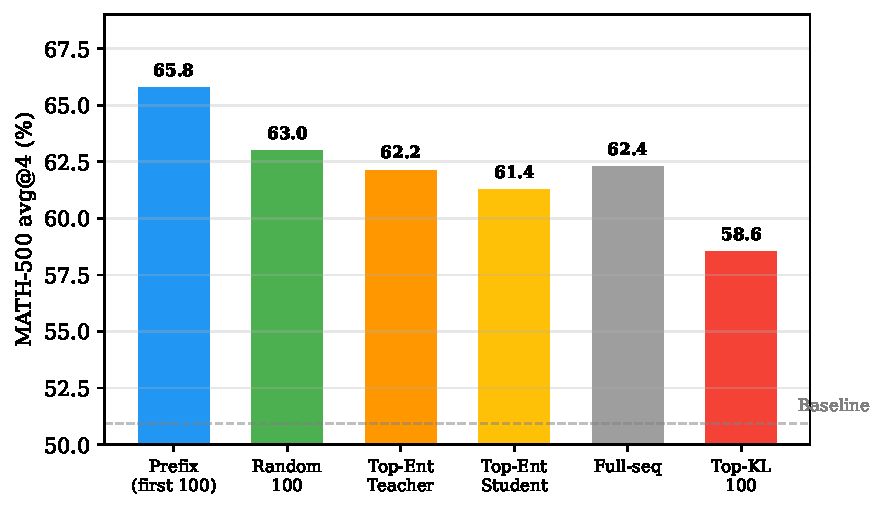
\includegraphics[width=0.8\columnwidth]{figures/fig_token_select.pdf}
    \caption{\textbf{Token selection strategies} ($k{=}100$, best avg@4). Prefix (first 100 tokens) outperforms all alternatives. Top-KL and top-entropy strategies select tokens with the highest signal concentration (95\%+ of total KL/entropy) but these tokens are at later positions (mean pos.\ 240--313) where the teacher signal is harmful. Random-100 outperforms all ``smart'' strategies except prefix by statistically avoiding later positions.}
    \label{fig:token_select}
\end{figure}

The results reveal a striking pattern: \textbf{the strategies that capture the most signal perform worst.} Top-KL-100 captures 95.6\% of total KL divergence yet achieves only 58.60\%---the worst of all methods. The key difference is \emph{position}: high-KL and high-entropy tokens are concentrated at later positions (mean position 240--313), while prefix tokens span positions 0--99. This confirms that \textbf{position is the most important criterion for token selection in on-policy distillation}.

\paragraph{LoRA vs.\ full fine-tuning.} LoRA ($r{=}32$) substantially outperforms full fine-tuning on both math (+9.7pp avg@4) and coding (+5.5pp HumanEval) for pos-100. Full results are in Appendix~\ref{app:full_results}.

\paragraph{Additional student-teacher pairs.} We evaluate with Qwen3-1.7B and Qwen3-4B as students (with 4B and 8B teachers). Distillation is most effective when the student has significant room for improvement: Qwen3-1.7B gains +13.9pp on BFCL from a 4B teacher. Stronger students show diminishing returns (Appendix~\ref{app:additional_pairs}).


% ============================================================================
% RELATED WORK
% ============================================================================
% =============================================================================
% related_work_section.tex --- Positional Distillation Paper
% Self-contained related work section (~1.5 pages)
% Usage: % =============================================================================
% related_work_section.tex --- Positional Distillation Paper
% Self-contained related work section (~1.5 pages)
% Usage: % =============================================================================
% related_work_section.tex --- Positional Distillation Paper
% Self-contained related work section (~1.5 pages)
% Usage: \input{related_work_section.tex} in main.tex
% =============================================================================

\section{Related Work}
\label{sec:related_work}

\paragraph{Knowledge Distillation for Language Models.}
Knowledge distillation~\citep{hinton2015distilling} transfers knowledge from a teacher model to a smaller student by training on soft targets.
\citet{kim2016sequence} extended this to sequence models with word-level and sequence-level distillation objectives.
For large language models, the choice of divergence measure and data distribution has proven critical.
\citet{gu2024minillm} demonstrated that reverse KL divergence is preferable for generative LLM distillation, as it avoids the student overestimating low-probability teacher modes.
\citet{agarwal2024onpolicy} introduced Generalized Knowledge Distillation (GKD), showing that on-policy generation---where the student generates sequences and the teacher provides soft labels---substantially outperforms supervised (off-policy) distillation.
\citet{ko2024distillm} proposed skew KL divergence and adaptive off-policy approaches for more efficient distillation, while \citet{wen2023fdivergence} generalized sequence-level KD to arbitrary f-divergences.
\citet{wu2025rethinking} challenged the conventional mode-seeking vs.\ mean-seeking interpretation of reverse and forward KL in the LLM setting, finding that both divergences converge given sufficient training but focus on different distribution regions in early epochs.
More recently, \citet{xu2025speculative} introduced Speculative Knowledge Distillation, which uses interleaved teacher-student sampling inspired by speculative decoding, filtering tokens the teacher is unlikely to produce.
Our work builds on the on-policy reverse KL paradigm of \citet{agarwal2024onpolicy} and \citet{gu2024minillm}, but introduces position-based loss computation that fundamentally changes which tokens receive gradient signal.

\paragraph{Token-Level Importance in Distillation and Reasoning.}
A growing body of work demonstrates that not all tokens contribute equally to learning.
\citet{wang2025beyond8020} showed that only $\sim$20\% of chain-of-thought tokens have high entropy, and these ``forking tokens'' steer reasoning paths---applying RL gradients to only these tokens matches full-gradient performance.
\citet{li2025preplan} discovered a ``preplan-and-anchor'' mechanism in LLM attention patterns, where models first perform long-range contextual reference before producing semantic anchor tokens, enabling targeted credit assignment.
\citet{singh2026functional} proposed greedy pruning of reasoning chains and showed that LLMs internally encode token-level functional importance for answer generation.

In the distillation setting specifically, several concurrent works have explored token selection.
\citet{huang2025selectkd} proposed SelecTKD, a propose-and-verify framework where the teacher verifies student-proposed tokens, applying full loss to accepted tokens and masking rejected ones.
\citet{xie2026adakd} introduced AdaKD, which adaptively adjusts token-level temperature based on learning stability.
\citet{tavor2026rethinking} systematically disentangled selective KD along position, class, and sample axes, proposing student-entropy-guided position selection (SE-KD) that reduces wall time by 70\% without sacrificing accuracy.
\citet{kim2026tsdkd} combined entropy-based token selection with preference ranking in a dual distillation framework.

Our approach differs from all of these in a fundamental way: we use \emph{absolute position} as the sole selection criterion, requiring no per-token computation of entropy, difficulty, or verification scores.
This simplicity is motivated by our empirical finding that KL divergence between teacher and student concentrates at early positions corresponding to reasoning strategy selection.
Furthermore, unlike prior token-selection methods that aim primarily at efficiency or robustness, we show that positional loss also eliminates training instability---a qualitative benefit that token-level adaptive methods do not address.

\paragraph{Training Stability and Sequence-Level Issues.}
Full-sequence on-policy distillation is known to suffer from instability.
\citet{holtzman2020curious} identified that likelihood-based training can produce bland, repetitive text---a form of neural text degeneration.
\citet{shumailov2024collapse} demonstrated that iteratively training generative models on their own outputs leads to model collapse, where distribution tails disappear.
In on-policy KD specifically, \citet{jang2026veto} proposed Veto, a geometric bridge in logit space that suppresses harmful gradients on low-confidence tokens, directly addressing the instability we also observe.
Our approach is complementary: rather than modifying the target distribution, we restrict the loss scope to early positions where teacher-student agreement is naturally highest, achieving stability through a simpler mechanism.

Several works have studied how sequence length affects distillation quality.
\citet{chen2025distillingessence} showed that training on only the first 50\% of tokens in supervised reasoning distillation retains $\sim$91\% of full-sequence performance, establishing a computation-quality tradeoff.
\citet{yan2026dasd} addressed exposure bias and capacity misalignment in long chain-of-thought distillation through temperature-scheduled learning.
Our work extends the truncation insight to the on-policy setting: we demonstrate that positional loss masking on student-generated sequences achieves equal or better performance than full-sequence loss, while providing the additional benefit of eliminating degenerate repetition patterns that are unique to on-policy training.

\paragraph{Curriculum Learning and Sequence Scheduling.}
Curriculum learning~\citep{bengio2009curriculum} improves training by gradually increasing task difficulty.
\citet{bengio2015scheduled} applied this principle to sequence models through scheduled sampling, transitioning from teacher-forced to free-running generation during training.
In the LLM pretraining setting, \citet{li2022stability} showed that long sequences at training start cause extreme gradient variance, and sequence length warmup stabilizes training while enabling larger batch sizes.
\citet{pouransari2024dataset} extended this with variable sequence length curriculum for LLM pretraining, achieving up to 3$\times$ faster convergence.
Our progressive position schedule---linearly increasing the position limit from 1 to 200 over training---applies the curriculum principle to the distillation loss scope rather than to the input sequence length, and represents a novel form of curriculum specific to knowledge distillation.

\paragraph{Mathematical Reasoning and Model Context.}
Our experiments use Qwen2.5-Math-1.5B~\citep{qwen2024qwen25math} as the student and Qwen3-1.7B~\citep{qwen2025qwen3} as the teacher, evaluating on the MATH-500 subset~\citep{lightman2023verify} of the MATH benchmark~\citep{hendrycks2021measuring}.
We use LoRA~\citep{hu2022lora} for parameter-efficient fine-tuning.
The distillation-vs-RL paradigm for reasoning has been established by DeepSeek-R1~\citep{deepseekr1}, which showed that distilled models can outperform RL-trained ones in certain settings.
Our work contributes to this landscape by demonstrating that the effectiveness of distillation can be significantly improved through principled control of the loss computation scope.
 in main.tex
% =============================================================================

\section{Related Work}
\label{sec:related_work}

\paragraph{Knowledge Distillation for Language Models.}
Knowledge distillation~\citep{hinton2015distilling} transfers knowledge from a teacher model to a smaller student by training on soft targets.
\citet{kim2016sequence} extended this to sequence models with word-level and sequence-level distillation objectives.
For large language models, the choice of divergence measure and data distribution has proven critical.
\citet{gu2024minillm} demonstrated that reverse KL divergence is preferable for generative LLM distillation, as it avoids the student overestimating low-probability teacher modes.
\citet{agarwal2024onpolicy} introduced Generalized Knowledge Distillation (GKD), showing that on-policy generation---where the student generates sequences and the teacher provides soft labels---substantially outperforms supervised (off-policy) distillation.
\citet{ko2024distillm} proposed skew KL divergence and adaptive off-policy approaches for more efficient distillation, while \citet{wen2023fdivergence} generalized sequence-level KD to arbitrary f-divergences.
\citet{wu2025rethinking} challenged the conventional mode-seeking vs.\ mean-seeking interpretation of reverse and forward KL in the LLM setting, finding that both divergences converge given sufficient training but focus on different distribution regions in early epochs.
More recently, \citet{xu2025speculative} introduced Speculative Knowledge Distillation, which uses interleaved teacher-student sampling inspired by speculative decoding, filtering tokens the teacher is unlikely to produce.
Our work builds on the on-policy reverse KL paradigm of \citet{agarwal2024onpolicy} and \citet{gu2024minillm}, but introduces position-based loss computation that fundamentally changes which tokens receive gradient signal.

\paragraph{Token-Level Importance in Distillation and Reasoning.}
A growing body of work demonstrates that not all tokens contribute equally to learning.
\citet{wang2025beyond8020} showed that only $\sim$20\% of chain-of-thought tokens have high entropy, and these ``forking tokens'' steer reasoning paths---applying RL gradients to only these tokens matches full-gradient performance.
\citet{li2025preplan} discovered a ``preplan-and-anchor'' mechanism in LLM attention patterns, where models first perform long-range contextual reference before producing semantic anchor tokens, enabling targeted credit assignment.
\citet{singh2026functional} proposed greedy pruning of reasoning chains and showed that LLMs internally encode token-level functional importance for answer generation.

In the distillation setting specifically, several concurrent works have explored token selection.
\citet{huang2025selectkd} proposed SelecTKD, a propose-and-verify framework where the teacher verifies student-proposed tokens, applying full loss to accepted tokens and masking rejected ones.
\citet{xie2026adakd} introduced AdaKD, which adaptively adjusts token-level temperature based on learning stability.
\citet{tavor2026rethinking} systematically disentangled selective KD along position, class, and sample axes, proposing student-entropy-guided position selection (SE-KD) that reduces wall time by 70\% without sacrificing accuracy.
\citet{kim2026tsdkd} combined entropy-based token selection with preference ranking in a dual distillation framework.

Our approach differs from all of these in a fundamental way: we use \emph{absolute position} as the sole selection criterion, requiring no per-token computation of entropy, difficulty, or verification scores.
This simplicity is motivated by our empirical finding that KL divergence between teacher and student concentrates at early positions corresponding to reasoning strategy selection.
Furthermore, unlike prior token-selection methods that aim primarily at efficiency or robustness, we show that positional loss also eliminates training instability---a qualitative benefit that token-level adaptive methods do not address.

\paragraph{Training Stability and Sequence-Level Issues.}
Full-sequence on-policy distillation is known to suffer from instability.
\citet{holtzman2020curious} identified that likelihood-based training can produce bland, repetitive text---a form of neural text degeneration.
\citet{shumailov2024collapse} demonstrated that iteratively training generative models on their own outputs leads to model collapse, where distribution tails disappear.
In on-policy KD specifically, \citet{jang2026veto} proposed Veto, a geometric bridge in logit space that suppresses harmful gradients on low-confidence tokens, directly addressing the instability we also observe.
Our approach is complementary: rather than modifying the target distribution, we restrict the loss scope to early positions where teacher-student agreement is naturally highest, achieving stability through a simpler mechanism.

Several works have studied how sequence length affects distillation quality.
\citet{chen2025distillingessence} showed that training on only the first 50\% of tokens in supervised reasoning distillation retains $\sim$91\% of full-sequence performance, establishing a computation-quality tradeoff.
\citet{yan2026dasd} addressed exposure bias and capacity misalignment in long chain-of-thought distillation through temperature-scheduled learning.
Our work extends the truncation insight to the on-policy setting: we demonstrate that positional loss masking on student-generated sequences achieves equal or better performance than full-sequence loss, while providing the additional benefit of eliminating degenerate repetition patterns that are unique to on-policy training.

\paragraph{Curriculum Learning and Sequence Scheduling.}
Curriculum learning~\citep{bengio2009curriculum} improves training by gradually increasing task difficulty.
\citet{bengio2015scheduled} applied this principle to sequence models through scheduled sampling, transitioning from teacher-forced to free-running generation during training.
In the LLM pretraining setting, \citet{li2022stability} showed that long sequences at training start cause extreme gradient variance, and sequence length warmup stabilizes training while enabling larger batch sizes.
\citet{pouransari2024dataset} extended this with variable sequence length curriculum for LLM pretraining, achieving up to 3$\times$ faster convergence.
Our progressive position schedule---linearly increasing the position limit from 1 to 200 over training---applies the curriculum principle to the distillation loss scope rather than to the input sequence length, and represents a novel form of curriculum specific to knowledge distillation.

\paragraph{Mathematical Reasoning and Model Context.}
Our experiments use Qwen2.5-Math-1.5B~\citep{qwen2024qwen25math} as the student and Qwen3-1.7B~\citep{qwen2025qwen3} as the teacher, evaluating on the MATH-500 subset~\citep{lightman2023verify} of the MATH benchmark~\citep{hendrycks2021measuring}.
We use LoRA~\citep{hu2022lora} for parameter-efficient fine-tuning.
The distillation-vs-RL paradigm for reasoning has been established by DeepSeek-R1~\citep{deepseekr1}, which showed that distilled models can outperform RL-trained ones in certain settings.
Our work contributes to this landscape by demonstrating that the effectiveness of distillation can be significantly improved through principled control of the loss computation scope.
 in main.tex
% =============================================================================

\section{Related Work}
\label{sec:related_work}

\paragraph{Knowledge Distillation for Language Models.}
Knowledge distillation~\citep{hinton2015distilling} transfers knowledge from a teacher model to a smaller student by training on soft targets.
\citet{kim2016sequence} extended this to sequence models with word-level and sequence-level distillation objectives.
For large language models, the choice of divergence measure and data distribution has proven critical.
\citet{gu2024minillm} demonstrated that reverse KL divergence is preferable for generative LLM distillation, as it avoids the student overestimating low-probability teacher modes.
\citet{agarwal2024onpolicy} introduced Generalized Knowledge Distillation (GKD), showing that on-policy generation---where the student generates sequences and the teacher provides soft labels---substantially outperforms supervised (off-policy) distillation.
\citet{ko2024distillm} proposed skew KL divergence and adaptive off-policy approaches for more efficient distillation, while \citet{wen2023fdivergence} generalized sequence-level KD to arbitrary f-divergences.
\citet{wu2025rethinking} challenged the conventional mode-seeking vs.\ mean-seeking interpretation of reverse and forward KL in the LLM setting, finding that both divergences converge given sufficient training but focus on different distribution regions in early epochs.
More recently, \citet{xu2025speculative} introduced Speculative Knowledge Distillation, which uses interleaved teacher-student sampling inspired by speculative decoding, filtering tokens the teacher is unlikely to produce.
Our work builds on the on-policy reverse KL paradigm of \citet{agarwal2024onpolicy} and \citet{gu2024minillm}, but introduces position-based loss computation that fundamentally changes which tokens receive gradient signal.

\paragraph{Token-Level Importance in Distillation and Reasoning.}
A growing body of work demonstrates that not all tokens contribute equally to learning.
\citet{wang2025beyond8020} showed that only $\sim$20\% of chain-of-thought tokens have high entropy, and these ``forking tokens'' steer reasoning paths---applying RL gradients to only these tokens matches full-gradient performance.
\citet{li2025preplan} discovered a ``preplan-and-anchor'' mechanism in LLM attention patterns, where models first perform long-range contextual reference before producing semantic anchor tokens, enabling targeted credit assignment.
\citet{singh2026functional} proposed greedy pruning of reasoning chains and showed that LLMs internally encode token-level functional importance for answer generation.

In the distillation setting specifically, several concurrent works have explored token selection.
\citet{huang2025selectkd} proposed SelecTKD, a propose-and-verify framework where the teacher verifies student-proposed tokens, applying full loss to accepted tokens and masking rejected ones.
\citet{xie2026adakd} introduced AdaKD, which adaptively adjusts token-level temperature based on learning stability.
\citet{tavor2026rethinking} systematically disentangled selective KD along position, class, and sample axes, proposing student-entropy-guided position selection (SE-KD) that reduces wall time by 70\% without sacrificing accuracy.
\citet{kim2026tsdkd} combined entropy-based token selection with preference ranking in a dual distillation framework.

Our approach differs from all of these in a fundamental way: we use \emph{absolute position} as the sole selection criterion, requiring no per-token computation of entropy, difficulty, or verification scores.
This simplicity is motivated by our empirical finding that KL divergence between teacher and student concentrates at early positions corresponding to reasoning strategy selection.
Furthermore, unlike prior token-selection methods that aim primarily at efficiency or robustness, we show that positional loss also eliminates training instability---a qualitative benefit that token-level adaptive methods do not address.

\paragraph{Training Stability and Sequence-Level Issues.}
Full-sequence on-policy distillation is known to suffer from instability.
\citet{holtzman2020curious} identified that likelihood-based training can produce bland, repetitive text---a form of neural text degeneration.
\citet{shumailov2024collapse} demonstrated that iteratively training generative models on their own outputs leads to model collapse, where distribution tails disappear.
In on-policy KD specifically, \citet{jang2026veto} proposed Veto, a geometric bridge in logit space that suppresses harmful gradients on low-confidence tokens, directly addressing the instability we also observe.
Our approach is complementary: rather than modifying the target distribution, we restrict the loss scope to early positions where teacher-student agreement is naturally highest, achieving stability through a simpler mechanism.

Several works have studied how sequence length affects distillation quality.
\citet{chen2025distillingessence} showed that training on only the first 50\% of tokens in supervised reasoning distillation retains $\sim$91\% of full-sequence performance, establishing a computation-quality tradeoff.
\citet{yan2026dasd} addressed exposure bias and capacity misalignment in long chain-of-thought distillation through temperature-scheduled learning.
Our work extends the truncation insight to the on-policy setting: we demonstrate that positional loss masking on student-generated sequences achieves equal or better performance than full-sequence loss, while providing the additional benefit of eliminating degenerate repetition patterns that are unique to on-policy training.

\paragraph{Curriculum Learning and Sequence Scheduling.}
Curriculum learning~\citep{bengio2009curriculum} improves training by gradually increasing task difficulty.
\citet{bengio2015scheduled} applied this principle to sequence models through scheduled sampling, transitioning from teacher-forced to free-running generation during training.
In the LLM pretraining setting, \citet{li2022stability} showed that long sequences at training start cause extreme gradient variance, and sequence length warmup stabilizes training while enabling larger batch sizes.
\citet{pouransari2024dataset} extended this with variable sequence length curriculum for LLM pretraining, achieving up to 3$\times$ faster convergence.
Our progressive position schedule---linearly increasing the position limit from 1 to 200 over training---applies the curriculum principle to the distillation loss scope rather than to the input sequence length, and represents a novel form of curriculum specific to knowledge distillation.

\paragraph{Mathematical Reasoning and Model Context.}
Our experiments use Qwen2.5-Math-1.5B~\citep{qwen2024qwen25math} as the student and Qwen3-1.7B~\citep{qwen2025qwen3} as the teacher, evaluating on the MATH-500 subset~\citep{lightman2023verify} of the MATH benchmark~\citep{hendrycks2021measuring}.
We use LoRA~\citep{hu2022lora} for parameter-efficient fine-tuning.
The distillation-vs-RL paradigm for reasoning has been established by DeepSeek-R1~\citep{deepseekr1}, which showed that distilled models can outperform RL-trained ones in certain settings.
Our work contributes to this landscape by demonstrating that the effectiveness of distillation can be significantly improved through principled control of the loss computation scope.



% ============================================================================
% DISCUSSION AND CONCLUSION
% ============================================================================
\section{Discussion}
\label{sec:discussion}

\paragraph{The conditional scoring problem is fundamental.} Our analysis reveals that a core issue in on-policy distillation is often overlooked: the teacher's supervision at position $t$ is not an unconditional assessment of token quality, but a \emph{conditional} assessment given the student's prefix $y_{<t}$. At early positions, this conditioning is minimal (the prefix is mostly the prompt), so the teacher provides genuinely independent guidance on reasoning strategy. At later positions, the teacher is locked into the student's chosen approach and can only score execution details within that approach. This ``conditional scoring problem'' explains both why early-position signal is valuable (it transfers strategy) and why later-position signal is harmful (it reinforces potentially suboptimal approaches).

\paragraph{Broader implications.} The signal quality degradation we identify may extend beyond distillation to other on-policy optimization methods that use token-level rewards, including RLHF and DPO. Whenever a reward model or reference model scores tokens conditioned on a learner-generated prefix, the same conditional dependency applies: later-position rewards are increasingly shaped by the learner's choices rather than representing independent quality assessments. Investigating positional signal quality in these settings is a promising direction.

\paragraph{Limitations.} Our signal quality analysis focuses on the Qwen model family; extending to other families and larger scales would validate generality. We evaluate only reverse KL divergence; forward KL or other $f$-divergences may show different positional patterns. The optimal $N$ varies by task (50--200 works broadly); adaptive per-example $N$ selection could be more robust.

\paragraph{Conclusion.} We show that in on-policy knowledge distillation, the teacher's per-token supervision quality is fundamentally non-uniform: early tokens carry strong, independent signal about reasoning strategy, while later tokens provide weak, dependent signal that is actively harmful when optimized. This insight motivates \methodfull{}---restricting KD loss to the first $N$ response tokens---which matches or exceeds full-sequence distillation across math, coding, and function calling tasks while eliminating training instability and achieving 20--35$\times$ speedup. Teaching the student how to begin is sufficient to improve the entire response.


% ============================================================================
% REFERENCES
% ============================================================================
\bibliographystyle{plainnat}
\bibliography{references_extended}


% ============================================================================
% APPENDIX
% ============================================================================
\appendix

\section{Training Efficiency}
\label{app:timing}

\begin{table}[!htbp]
\centering
\caption{\textbf{Per-step time breakdown.} Wall-clock time on a single A6000 (48GB). Student: Qwen2.5-Math-1.5B, LoRA, bs=16.}
\label{tab:timing_detailed}
\small
\begin{tabular}{llcccc}
\toprule
\textbf{Teacher} & \textbf{Method} & \textbf{Gen (s)} & \textbf{Score (s)} & \textbf{Train (s)} & \textbf{Total (s)} \\
\midrule
\multirow{2}{*}{Q3-1.7B} & Full-seq & 100--731 & 3--10 & 5--12 & ${\sim}$280 \\
 & Ours ($N{=}100$) & ${\sim}$5 & ${\sim}$1 & ${\sim}$2 & ${\sim}$8 \\
\midrule
\multirow{2}{*}{Q3-4B} & Full-seq & 97--733 & 3--9 & 6--10 & ${\sim}$210 \\
 & Ours ($N{=}100$) & ${\sim}$5 & ${\sim}$1 & ${\sim}$2 & ${\sim}$8 \\
\midrule
\multirow{2}{*}{Q3-8B} & Full-seq & 96--230 & 7--11 & 1--6 & ${\sim}$170$^\dagger$ \\
 & Ours ($N{=}100$) & ${\sim}$5 & ${\sim}$1 & ${\sim}$2 & ${\sim}$8 \\
\bottomrule
\multicolumn{6}{l}{\footnotesize $^\dagger$ Frequent OOMs; 48GB insufficient for 8B teacher + vLLM + student.}
\end{tabular}
\end{table}


\section{Additional Student-Teacher Pairs}
\label{app:additional_pairs}

\begin{table}[!htbp]
\centering
\caption{\textbf{Additional student-teacher pairs.} All use pos-100, LoRA, 3,200 problems.}
\label{tab:additional_pairs}
\small
\begin{tabular}{llccc}
\toprule
\textbf{Student} & \textbf{Teacher} & \textbf{MATH-500 avg@4} & \textbf{BFCL full\_acc} & \textbf{HumanEval pass@1} \\
\midrule
Qwen3-1.7B & --- (baseline) & 69.20\% & 59.80\% & 39.63\% \\
Qwen3-1.7B & Qwen3-4B & 69.20\% & 73.70\% & 44.51\% \\
Qwen3-1.7B & Qwen3-8B & 69.15\% & 74.00\% & 40.24\% \\
\midrule
Qwen3-4B & --- (baseline) & 77.95\% & 73.00\% & 73.17\% \\
Qwen3-4B & Qwen3-8B & 77.05\% & 76.80\% & 71.34\% \\
\bottomrule
\end{tabular}
\end{table}


\section{Full Experimental Results}
\label{app:full_results}

\subsection{Math Results: Per-Step Performance}

Table~\ref{tab:app_math_main} presents per-step results for the primary math experiments (LoRA, $n{=}1$, 3,200 problems).

\begin{table}[!htbp]
\centering
\caption{\textbf{MATH-500 per-step results.} LoRA, $n{=}1$, $\text{bs}{=}16$, 3,200 problems. Baseline: 50.95\% avg@4.}
\label{tab:app_math_main}
\small
\begin{tabular}{ll cccc}
\toprule
\textbf{Method} & \textbf{Metric} & \textbf{Step 50} & \textbf{Step 100} & \textbf{Step 150} & \textbf{Step 200} \\
\midrule
\multirow{3}{*}{Pos-50} & avg@4 & 62.35 & 66.05 & \textbf{66.65} & 64.85 \\
 & maj@4 & 69.40 & 72.00 & 71.00 & 71.20 \\
 & pass@4 & 77.20 & 79.40 & 81.00 & 79.60 \\
\midrule
\multirow{3}{*}{Pos-100} & avg@4 & 63.75 & 64.45 & 65.15 & \textbf{65.85} \\
 & maj@4 & 70.00 & 68.40 & 69.60 & 70.80 \\
 & pass@4 & 79.80 & 78.40 & 80.20 & 79.80 \\
\midrule
\multirow{3}{*}{Pos-150} & avg@4 & 65.35 & \textbf{66.65} & 65.30 & 65.75 \\
 & maj@4 & 66.80 & 67.00 & 66.30 & 67.30 \\
 & pass@4 & 79.00 & 81.00 & 78.20 & 80.00 \\
\midrule
\multirow{3}{*}{Pos-200} & avg@4 & \textbf{66.05} & 64.65 & 65.10 & 65.55 \\
 & maj@4 & 71.20 & 68.40 & 70.00 & 71.20 \\
 & pass@4 & 81.00 & 79.80 & 80.60 & 80.60 \\
\bottomrule
\end{tabular}
\end{table}


\subsection{Math Results: Earlier Series ($n{=}16$, 200 problems)}

\begin{table}[!htbp]
\centering
\caption{\textbf{Complete MATH-500 results, LoRA, $n{=}16$, $\text{bs}{=}16$.} Best per configuration in \textbf{bold}.}
\label{tab:app_math_n16}
\footnotesize
\begin{tabular}{lcccc}
\toprule
\textbf{Config} & \textbf{Step 50} & \textbf{Step 100} & \textbf{Step 150} & \textbf{Step 200} \\
\midrule
\multicolumn{5}{l}{\textit{avg@4}} \\
\midrule
Pos-5 & 55.15 & 55.65 & \textbf{56.50} & 56.30 \\
Pos-10 & \textbf{59.50} & 56.40 & 56.30 & 56.00 \\
Pos-20 & \textbf{60.20} & 57.35 & 56.40 & 56.55 \\
Pos-50 & \textbf{62.45} & 62.15 & 60.50 & 61.90 \\
Pos-100 & 61.15 & 63.55 & \textbf{64.25} & 63.85 \\
Pos-150 & 63.55 & \textbf{65.70} & 64.80 & 64.40 \\
Pos-200 & 63.25 & \textbf{66.75} & 64.55 & 65.25 \\
Progressive & 61.10 & 62.05 & 61.95 & \textbf{62.30} \\
Full-seq$^\dagger$ & \textbf{65.60} & 46.30 & 49.70 & 43.80 \\
Full-seq (first-boxed) & \textbf{65.55} & 64.95 & 65.55 & 64.95 \\
\midrule
\multicolumn{5}{l}{\textit{pass@4}} \\
\midrule
Pos-5 & 74.0 & 74.8 & \textbf{76.0} & 73.4 \\
Pos-10 & \textbf{75.8} & 73.2 & 75.4 & 74.2 \\
Pos-20 & \textbf{77.0} & 76.0 & 73.4 & 75.8 \\
Pos-50 & 77.0 & 78.4 & 77.6 & \textbf{78.6} \\
Pos-100 & 77.6 & 79.2 & \textbf{80.2} & 80.2 \\
Pos-150 & 79.6 & 77.4 & \textbf{80.0} & 79.4 \\
Pos-200 & 79.6 & \textbf{80.2} & 79.4 & 79.2 \\
Progressive & 77.2 & 77.8 & 78.2 & \textbf{78.8} \\
Full-seq & \textbf{80.0} & 72.2 & 77.0 & 74.2 \\
\bottomrule
\multicolumn{5}{l}{\footnotesize $^\dagger$ Last-boxed extraction; degrades due to repetition.}
\end{tabular}
\end{table}


\subsection{Coding Results}

\begin{table}[!htbp]
\centering
\caption{\textbf{Complete coding results, LoRA.} HumanEval (HE) and MBPP pass@1.}
\label{tab:app_coding_lora}
\footnotesize
\begin{tabular}{llcccccccc}
\toprule
\textbf{Config} & \textbf{Metric} & \textbf{s50} & \textbf{s100} & \textbf{s150} & \textbf{s200} & \textbf{s250} & \textbf{s300} & \textbf{s350} & \textbf{s400} \\
\midrule
\multirow{2}{*}{Pos-50} & HE & 37.8 & 39.0 & 39.6 & 41.5 & 40.2 & 40.9 & \textbf{42.1} & 40.9 \\
 & MBPP & 52.1 & 48.9 & 46.0 & 46.0 & 47.6 & 46.3 & 46.6 & 46.3 \\
\midrule
\multirow{2}{*}{Pos-100} & HE & 37.2 & 39.0 & \textbf{42.1} & 37.8 & 39.0 & 37.8 & 37.8 & 38.4 \\
 & MBPP & 52.1 & 49.7 & 49.2 & 49.2 & 48.4 & 49.2 & 47.9 & 48.9 \\
\midrule
\multirow{2}{*}{Pos-150} & HE & 36.6 & 35.4 & 36.6 & 39.0 & \textbf{41.5} & 39.6 & 38.4 & 37.2 \\
 & MBPP & 51.3 & 50.0 & 48.4 & 50.5 & 49.5 & 50.3 & 49.7 & 48.7 \\
\midrule
\multirow{2}{*}{Full-seq} & HE & \textbf{40.2} & 31.7 & 32.3 & 32.9 & 27.4 & 28.0 & 26.8 & 26.8 \\
 & MBPP & 52.6 & 48.9 & 49.5 & 48.1 & 47.9 & 47.1 & 48.4 & 47.6 \\
\bottomrule
\end{tabular}
\end{table}


\subsection{Full Fine-Tuning Results}

\begin{table}[!htbp]
\centering
\caption{\textbf{MATH-500 per-step results, full fine-tuning.} $n{=}1$, $\text{bs}{=}16$, 3,200 problems, lr=$5{\times}10^{-6}$. Baseline: 50.95\% avg@4.}
\label{tab:app_math_fullft}
\small
\begin{tabular}{ll cccc}
\toprule
\textbf{Method} & \textbf{Metric} & \textbf{Step 50} & \textbf{Step 100} & \textbf{Step 150} & \textbf{Step 200} \\
\midrule
\multirow{3}{*}{Pos-50} & avg@4 & 55.55 & 55.85 & \textbf{56.75} & 55.50 \\
 & maj@4 & 65.20 & 65.00 & 66.20 & 64.20 \\
 & pass@4 & 75.60 & 74.40 & 74.80 & 75.00 \\
\midrule
\multirow{3}{*}{Pos-100} & avg@4 & 55.15 & \textbf{56.20} & 55.65 & 54.80 \\
 & maj@4 & 64.00 & 64.20 & 64.60 & 63.00 \\
 & pass@4 & 74.00 & 73.80 & 74.20 & 74.20 \\
\midrule
\multirow{3}{*}{Pos-200} & avg@4 & 55.45 & 55.80 & 55.90 & \textbf{56.40} \\
 & maj@4 & 64.40 & 64.00 & 64.00 & 65.20 \\
 & pass@4 & 74.60 & 74.80 & 75.60 & 75.20 \\
\midrule
\multirow{3}{*}{Full-seq} & avg@4 & 53.75 & 56.95 & 57.55 & \textbf{58.20} \\
 & maj@4 & 61.00 & 66.80 & 65.80 & 65.40 \\
 & pass@4 & 73.40 & 77.40 & 75.60 & 75.40 \\
\bottomrule
\end{tabular}
\end{table}

\begin{table}[!htbp]
\centering
\caption{\textbf{Coding results, full fine-tuning.} HumanEval (HE) and MBPP pass@1. $n{=}1$, $\text{bs}{=}16$, 6,400 problems, lr=$5{\times}10^{-6}$.}
\label{tab:app_coding_fullft}
\footnotesize
\begin{tabular}{llcccccccc}
\toprule
\textbf{Config} & \textbf{Metric} & \textbf{s50} & \textbf{s100} & \textbf{s150} & \textbf{s200} & \textbf{s250} & \textbf{s300} & \textbf{s350} & \textbf{s400} \\
\midrule
\multirow{2}{*}{Pos-50} & HE & 31.7 & 35.4 & \textbf{36.0} & 36.0 & 36.0 & 35.4 & 36.0 & 34.8 \\
 & MBPP & 52.6 & \textbf{53.4} & 52.9 & 52.4 & 52.4 & 52.6 & 52.9 & 53.4 \\
\midrule
\multirow{2}{*}{Pos-100} & HE & 31.7 & 34.1 & 35.4 & 34.8 & \textbf{36.6} & 36.0 & 36.0 & 36.6 \\
 & MBPP & 52.6 & \textbf{54.0} & 52.6 & 52.1 & 53.2 & 53.4 & 53.4 & 52.9 \\
\midrule
\multirow{2}{*}{Pos-150} & HE & 31.7 & 36.0 & 36.0 & 35.4 & 36.0 & 36.6 & 35.4 & \textbf{37.2} \\
 & MBPP & 53.2 & 51.9 & 52.4 & 52.4 & 53.2 & \textbf{54.2} & 53.2 & 52.4 \\
\midrule
\multirow{2}{*}{Pos-250} & HE & 32.9 & 34.8 & 35.4 & 35.4 & 37.2 & 36.6 & \textbf{37.8} & 33.5 \\
 & MBPP & 54.0 & 53.7 & 54.0 & \textbf{54.8} & 54.5 & 53.4 & 54.2 & 53.2 \\
\midrule
\multirow{2}{*}{Pos-200tok} & HE & 32.3 & \textbf{36.6} & 36.6 & 35.4 & 36.0 & 34.8 & 36.0 & 35.4 \\
 & MBPP & 52.1 & 52.6 & 54.0 & 52.6 & 53.7 & \textbf{54.5} & 53.2 & 53.7 \\
\midrule
\multirow{2}{*}{Full-seq} & HE & 32.3 & 32.3 & \textbf{36.6} & 36.0 & 31.1 & 30.5 & 31.7 & 31.1 \\
 & MBPP & 53.2 & 53.4 & 53.2 & \textbf{54.0} & 51.9 & 52.9 & 52.9 & 53.7 \\
\bottomrule
\end{tabular}
\end{table}


\subsection{Function Calling Results}

\begin{table}[!htbp]
\centering
\caption{\textbf{Function calling results (BFCL), LoRA.} Name accuracy / Full accuracy / Parse rate. Best full\_acc in \textbf{bold}.}
\label{tab:app_funcall}
\small
\begin{tabular}{lccccc}
\toprule
\textbf{Method} & \textbf{Best Step} & \textbf{Name Acc} & \textbf{Full Acc} & \textbf{Parse Rate} \\
\midrule
Baseline & --- & 9.70\% & 2.70\% & 24.20\% \\
Teacher (Qwen3-1.7B) & --- & 75.30\% & 54.00\% & 75.30\% \\
\midrule
Pos-50 & 200 & 95.20\% & 57.20\% & 98.30\% \\
\textbf{Pos-100} & \textbf{100} & 86.20\% & \textbf{61.30\%} & 91.30\% \\
Pos-150 & 200 & 88.70\% & 61.50\% & 92.50\% \\
Pos-200 & 200 & 80.80\% & 54.50\% & 90.20\% \\
Full-seq & 100 & 81.00\% & 58.20\% & 86.70\% \\
\bottomrule
\end{tabular}
\end{table}


\subsection{Scaling Experiment Results}

\begin{table}[!htbp]
\centering
\caption{\textbf{Scaling results.} All use pos-100, LoRA, 3,200 problems. Best across training steps. Baseline performance shown for reference.}
\label{tab:app_scaling}
\small
\begin{tabular}{llccc}
\toprule
\textbf{Student $\rightarrow$ Teacher} & \textbf{Math avg@4} & \textbf{BFCL full\_acc} & \textbf{HE pass@1} & \textbf{MBPP+ pass@1} \\
\midrule
M-1.5B baseline & 50.95\% & 2.70\% & --- & --- \\
M-1.5B $\rightarrow$ Q3-1.7B & 65.85\% & 61.30\% & 42.07\% & 44.44\% \\
M-1.5B $\rightarrow$ Q3-4B & 68.95\% & 45.80\% & 43.29\% & 47.62\% \\
M-1.5B $\rightarrow$ Q3-8B & 67.85\% & 57.00\% & 41.46\% & 44.44\% \\
\midrule
Q3-1.7B baseline & 69.20\% & 59.80\% & 39.63\% & 44.71\% \\
Q3-1.7B $\rightarrow$ Q3-4B & 69.20\% & 73.70\% & 44.51\% & 47.62\% \\
Q3-1.7B $\rightarrow$ Q3-8B & 69.15\% & 74.00\% & 40.24\% & 48.15\% \\
\midrule
Q3-4B baseline & 77.95\% & 73.00\% & 73.17\% & 55.56\% \\
Q3-4B $\rightarrow$ Q3-8B & 77.05\% & 76.80\% & 71.34\% & 56.35\% \\
\bottomrule
\end{tabular}
\end{table}


\subsection{Full-Sequence Degradation Details}
\label{app:fullseq_degradation}

\begin{table}[!htbp]
\centering
\caption{\textbf{Boxed repetition progression} in full-sequence LoRA distillation on MATH-500 ($n{=}16$, $\text{bs}{=}16$).}
\label{tab:app_boxed}
\small
\begin{tabular}{lcccc}
\toprule
\textbf{Statistic} & \textbf{Step 50} & \textbf{Step 100} & \textbf{Step 150} & \textbf{Step 200} \\
\midrule
Multi-boxed responses & 2.9\% & 91.5\% & 80.5\% & 89.1\% \\
Avg \bboxed{} per response & 1.0 & 88.1 & 54.1 & 58.0 \\
Repetitive responses & 5.9\% & 78.8\% & 58.3\% & 77.5\% \\
Avg response length (chars) & 1,388 & 4,023 & 3,585 & 4,558 \\
\midrule
Official avg@4 & 65.60\% & 46.30\% & 49.70\% & 43.80\% \\
Relaxed avg@4 (GT in text) & 74.60\% & 70.90\% & 71.90\% & 70.30\% \\
\bottomrule
\end{tabular}
\end{table}


\section{Token Classification Methodology}
\label{app:token_classification}

We classify each token into six categories based on string matching:
\begin{enumerate}
    \item \textbf{planning}: Reasoning keywords (``To'', ``Let'', ``First'', ``Step'', ``We'', ``Given'', ``Therefore'', ``Thus'', ``Since'').
    \item \textbf{structural}: Punctuation, whitespace, formatting tokens.
    \item \textbf{math\_number}: Digits (0--9).
    \item \textbf{math\_operator}: Arithmetic operators ($+$, $-$, $\times$, $/$, $=$).
    \item \textbf{math\_latex}: LaTeX delimiters (\texttt{\textbackslash(}, \texttt{\textbackslash[}).
    \item \textbf{continuation}: All others.
\end{enumerate}

\begin{table}[!htbp]
\centering
\caption{\textbf{Mean KL by token category and position range.}}
\label{tab:app_kl_by_category}
\small
\begin{tabular}{lcccccc}
\toprule
\textbf{Category} & \textbf{0--4} & \textbf{5--19} & \textbf{20--49} & \textbf{50--99} & \textbf{100--199} & \textbf{200--499} \\
\midrule
planning & 4.50 & 0.79 & 1.49 & 1.66 & 1.49 & 2.37 \\
structural & 3.26 & 1.46 & 1.60 & 0.93 & 0.60 & 0.86 \\
math\_number & 1.49 & 0.60 & 0.74 & 0.28 & 0.17 & 0.13 \\
math\_operator & 7.30 & 1.84 & 0.81 & 0.37 & 0.21 & 0.14 \\
math\_latex & 8.84 & 9.23 & 6.50 & 4.95 & 2.97 & 1.87 \\
continuation & 1.94 & 1.12 & 1.19 & 0.89 & 0.70 & 0.48 \\
\bottomrule
\end{tabular}
\end{table}

\begin{table}[!htbp]
\centering
\caption{\textbf{Top 20 highest-KL tokens} (minimum 50 occurrences across 10,000 trajectories).}
\label{tab:app_high_kl_tokens}
\small
\begin{tabular}{clccc}
\toprule
\textbf{Rank} & \textbf{Token} & \textbf{Category} & \textbf{Count} & \textbf{Mean KL} \\
\midrule
1 & ``Solution'' & planning & 152 & 21.93 \\
2 & ``Analysis'' & continuation & 125 & 16.49 \\
3 & \texttt{\textbackslash[} & math\_latex & 7,152 & 13.21 \\
4 & ``examines'' & continuation & 74 & 11.51 \\
5 & ``He'' & continuation & 150 & 10.80 \\
6 & \texttt{\textbackslash(} & math\_latex & 21,243 & 10.30 \\
7 & ``First'' & planning & 1,706 & 9.98 \\
8 & ``tests'' & continuation & 52 & 8.71 \\
9 & \texttt{\textbackslash\textbackslash} & math\_latex & 82 & 8.68 \\
10 & ``There'' & continuation & 201 & 8.28 \\
11 & ``Therefore'' & planning & 4,913 & 7.95 \\
12 & ``Identify'' & continuation & 1,345 & 7.78 \\
13 & ``To'' & planning & 8,806 & 6.90 \\
14 & ``When'' & continuation & 89 & 6.62 \\
15 & ``This'' & continuation & 621 & 6.34 \\
16 & ``Thus'' & planning & 2,547 & 6.24 \\
17 & ``First'' (space) & planning & 259 & 6.10 \\
18 & ``To'' (space) & planning & 1,174 & 5.37 \\
19 & ``The'' & planning & 2,626 & 5.25 \\
20 & ``Next'' & planning & 1,753 & 5.03 \\
\bottomrule
\end{tabular}
\end{table}


\end{document}
